\documentclass[10pt]{article}
\usepackage{xcolor}

\usepackage{listings}

\usepackage{geometry}
% NCE maximal width is 15 cm
\geometry{paperwidth=3.5in, paperheight=2.65in, top=0pt, bottom=0pt, right=0pt, left=0pt}
\usepackage{tikz}
\usetikzlibrary{arrows, calc, patterns, decorations.pathmorphing, fit, positioning, shapes.misc}


\def\grid{7}        % grid size (mm)
\def\laneGap{2}     % gap between lanes (mm)
\def\ellipsisGap{5} % gap to last lane (mm)

\begin{document}
\begin{tikzpicture}

    %--------------------------------------------------------
    % Sparse
    %--------------------------------------------------------
    \node (block_sparse) at (0, 0){
        \begin{tikzpicture}
            % Axis label
            \pgfmathtruncatemacro{\laneHeight}{8 * \grid}
            \node at ({-0.5 * \grid mm}, {\laneHeight mm + (\grid mm / 2)}) {A};

            % Draw first lanes
            \foreach \j in {0,...,1} {
                \pgfmathtruncatemacro{\laneStart}{\j * (\laneGap + \grid)}

                % Draw thread lines
                \draw [<-,decorate,decoration={
                    snake,amplitude=\grid/0.8 mm,pre length=\grid/0.5 mm, post length=0 mm}]
                    ({\laneStart mm + (\grid mm / 2)},  {\laneHeight mm + (0.1 * \grid mm)})
                    --
                    + (0, \grid mm);

                % Draw boxes and labels
                \foreach \i in {0,...,7} {
                    \pgfmathtruncatemacro{\index}{\j + (32 * (7 - \i))}

                    \draw (\laneStart mm, \grid mm * \i) +(0,0) rectangle ++(\grid mm,\grid mm);
                    \node at ({\laneStart mm + (\grid mm / 2)},  {\grid mm * (\i + 0.5)}) {$i_{\index}$};
                }
            }
            
            % Draw last lane
            \pgfmathtruncatemacro{\lastLaneStart}{(2 * (\laneGap + \grid)) + \ellipsisGap}

             % Draw thread line
                \draw [<-,decorate,decoration={
                    snake,amplitude=\grid/0.8 mm,pre length=\grid/0.5 mm, post length=0 mm}]
                    ({\lastLaneStart mm + (\grid mm / 2)},  {\laneHeight mm + (0.1 * \grid mm)})
                    --
                    + (0, \grid mm);

            \foreach \i in {0,...,7} {
                \pgfmathtruncatemacro{\index}{31 + (32 * (7 - \i))}

                % Boxes
                \draw (\lastLaneStart mm, \grid mm * \i) +(0,0) rectangle ++(\grid mm,\grid mm);
                
                % Labels
                \node at ({\lastLaneStart mm + (\grid mm / 2)},  {\grid mm * (\i + 0.5)}) {$i_{\index}$};
                
                % Ellipsis between continuous and last nodex
                \node at ({\lastLaneStart mm - (\ellipsisGap mm / 2) - 0.5 mm},  {\grid mm * (\i + 0.5)}) {\ldots};
            }

        \end{tikzpicture}
    };
    
    %--------------------------------------------------------
    % Delayed
    %--------------------------------------------------------
    \node (block_delay) at (40mm, 0){
        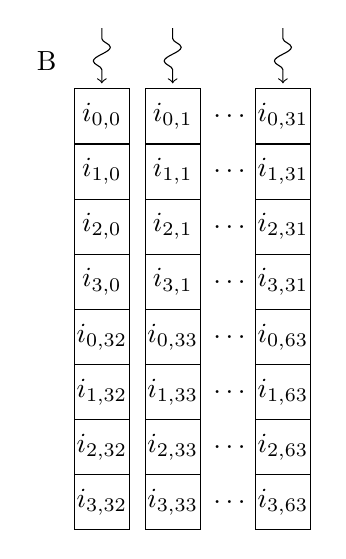
\begin{tikzpicture}
            % Axis label
            \pgfmathtruncatemacro{\laneHeight}{8 * \grid}
            \node at ({-0.5 * \grid mm}, {\laneHeight mm + (\grid mm / 2)}) {B};

            % Draw first lanes
            \foreach \j in {0,...,1} {
                \pgfmathtruncatemacro{\laneStart}{\j * (\laneGap + \grid)}

                % Draw thread lines
                \draw [<-,decorate,decoration={
                    snake,amplitude=\grid/0.8 mm,pre length=\grid/0.5 mm, post length=0 mm}]
                    ({\laneStart mm + (\grid mm / 2)},  {\laneHeight mm + (0.1 * \grid mm)})
                    --
                    + (0, \grid mm);

                % Draw labels
                \foreach \i in {0,...,1} {
                    \foreach \d in {0,...,3} {
                        \pgfmathtruncatemacro{\y}{(\i * 4) + \d}
                        \pgfmathtruncatemacro{\delay}{(3 - \d)}
                        \pgfmathtruncatemacro{\index}{\j + (32 * (1 - \i))}
                        \draw (\laneStart mm, \grid mm * \y) +(0,0) rectangle ++(\grid mm,\grid mm);
                        \node at ({\laneStart mm + (\grid mm / 2)},  {\grid mm * (\y + 0.5)}) {$i_{\delay, \index}$};
                    }
                }    
            }
            
            % Draw last lane
            \pgfmathtruncatemacro{\lastLaneStart}{(2 * (\laneGap + \grid)) + \ellipsisGap}

             % Draw thread line
                \draw [<-,decorate,decoration={
                    snake,amplitude=\grid/0.8 mm,pre length=\grid/0.5 mm, post length=0 mm}]
                    ({\lastLaneStart mm + (\grid mm / 2)},  {\laneHeight mm + (0.1 * \grid mm)})
                    --
                    + (0, \grid mm);

            % Draw labels
            \foreach \i in {0,...,1} {
                \foreach \d in {0,...,3} {
                    \pgfmathtruncatemacro{\y}{(\i * 4) + \d}
                    \pgfmathtruncatemacro{\delay}{(3 - \d)}
                    \pgfmathtruncatemacro{\index}{31 + (32 * (1 - \i))}

                    % Box
                    \draw (\lastLaneStart mm, \grid mm * \y) +(0,0) rectangle ++(\grid mm,\grid mm);

                    % Labels
                    \node at ({\lastLaneStart mm + (\grid mm / 2)},  {\grid mm * (\y + 0.5)}) {$i_{\delay, \index}$};
  
                    % Ellipsis
                    \node at ({\lastLaneStart mm - (\ellipsisGap mm / 2) - 0.5 mm},  {\grid mm * (\y + 0.5)}) {\ldots};
                }
            }

        \end{tikzpicture}
    };

\end{tikzpicture}
\end{document}
